\documentclass[usenames,dvipsnames]{beamer}
\usepackage{../../shared/styles/custom}
% =============================================================================
% ML TEACHING MATHEMATICAL NOTATION CONVENTIONS
% =============================================================================
% Based on standard ML textbooks: Murphy's "Machine Learning: A Probabilistic Perspective",
% Bishop's "Pattern Recognition and Machine Learning", and "Mathematics for Machine Learning"

% =============================================================================
% CORE NOTATION STANDARDS
% =============================================================================

% SCALARS: Regular italics (lowercase for variables, uppercase for constants)
% Examples: x, y, n, d, k, \theta, \alpha, \lambda, \sigma

% VECTORS: Bold lowercase letters
% Examples: \mathbf{x}, \mathbf{w}, \mathbf{\mu}, \mathbf{\theta}

% MATRICES: Bold uppercase letters
% Examples: \mathbf{X}, \mathbf{W}, \mathbf{\Sigma}, \mathbf{\Lambda}

% SETS: Calligraphic uppercase
% Examples: \mathcal{D}, \mathcal{X}, \mathcal{Y}

% SPACES: Blackboard bold
% Examples: \mathbb{R}, \mathbb{Z}, \mathbb{N}

% =============================================================================
% VECTOR NOTATION (bold lowercase)
% =============================================================================

\newcommand{\vx}{\mathbf{x}}        % Input vector
\newcommand{\vy}{\mathbf{y}}        % Output vector
\newcommand{\vw}{\mathbf{w}}        % Weight vector
\newcommand{\vb}{\mathbf{b}}        % Bias vector
\newcommand{\vh}{\mathbf{h}}        % Hidden vector
\newcommand{\vz}{\mathbf{z}}        % Latent vector
\newcommand{\vf}{\mathbf{f}}        % Function vector
\newcommand{\vg}{\mathbf{g}}        % Gradient vector
\newcommand{\vu}{\mathbf{u}}        % Generic vector u
\newcommand{\vv}{\mathbf{v}}        % Generic vector v
\newcommand{\vzero}{\mathbf{0}}     % Zero vector
\newcommand{\vone}{\mathbf{1}}      % Ones vector

% Greek vectors (bold)
\newcommand{\vmu}{\boldsymbol{\mu}}     % Mean vector
\newcommand{\vtheta}{\boldsymbol{\theta}} % Parameter vector
\newcommand{\vlambda}{\boldsymbol{\lambda}} % Lambda vector
\newcommand{\valpha}{\boldsymbol{\alpha}}   % Alpha vector
\newcommand{\vbeta}{\boldsymbol{\beta}}     % Beta vector
\newcommand{\vxi}{\boldsymbol{\xi}}         % Xi vector
\newcommand{\vepsilon}{\boldsymbol{\epsilon}} % Epsilon vector

% =============================================================================
% MATRIX NOTATION (bold uppercase)
% =============================================================================

\newcommand{\mX}{\mathbf{X}}        % Data matrix
\newcommand{\mY}{\mathbf{Y}}        % Target matrix
\newcommand{\mW}{\mathbf{W}}        % Weight matrix
\newcommand{\mA}{\mathbf{A}}        % Generic matrix A
\newcommand{\mB}{\mathbf{B}}        % Generic matrix B
\newcommand{\mC}{\mathbf{C}}        % Generic matrix C
\newcommand{\mH}{\mathbf{H}}        % Hidden layer matrix / Hessian
\newcommand{\mI}{\mathbf{I}}        % Identity matrix
\newcommand{\mJ}{\mathbf{J}}        % Jacobian matrix
\newcommand{\mK}{\mathbf{K}}        % Kernel matrix
\newcommand{\mL}{\mathbf{L}}        % Loss matrix / Cholesky factor
\newcommand{\mP}{\mathbf{P}}        % Projection matrix
\newcommand{\mQ}{\mathbf{Q}}        % Orthogonal matrix
\newcommand{\mR}{\mathbf{R}}        % Rotation matrix
\newcommand{\mS}{\mathbf{S}}        % Scatter matrix
\newcommand{\mU}{\mathbf{U}}        % Left singular vectors
\newcommand{\mV}{\mathbf{V}}        % Right singular vectors

% Greek matrices (bold)
\newcommand{\mSigma}{\boldsymbol{\Sigma}}   % Covariance matrix
\newcommand{\mLambda}{\boldsymbol{\Lambda}} % Diagonal eigenvalue matrix
\newcommand{\mPhi}{\boldsymbol{\Phi}}       % Feature matrix
\newcommand{\mPsi}{\boldsymbol{\Psi}}       % Basis matrix
\newcommand{\mTheta}{\boldsymbol{\Theta}}   % Parameter matrix

% =============================================================================
% SETS AND SPACES (following Bishop/Murphy conventions)
% =============================================================================

\newcommand{\cD}{\mathcal{D}}       % Dataset
\newcommand{\cH}{\mathcal{H}}       % Hypothesis space
\newcommand{\cX}{\mathcal{X}}       % Input space
\newcommand{\cY}{\mathcal{Y}}       % Output space
\newcommand{\cF}{\mathcal{F}}       % Function space
\newcommand{\cG}{\mathcal{G}}       % Gaussian process
\newcommand{\cL}{\mathcal{L}}       % Lagrangian / Loss
\newcommand{\cN}{\mathcal{N}}       % Normal distribution
\newcommand{\cU}{\mathcal{U}}       % Uniform distribution
\newcommand{\cB}{\mathcal{B}}       % Bernoulli distribution
\newcommand{\cP}{\mathcal{P}}       % Probability distribution

% Number systems
\newcommand{\Real}{\mathbb{R}}      % Real numbers
\newcommand{\Nat}{\mathbb{N}}       % Natural numbers
\newcommand{\Int}{\mathbb{Z}}       % Integers
\newcommand{\Complex}{\mathbb{C}}   % Complex numbers

% =============================================================================
% OPERATORS AND FUNCTIONS (following standard conventions)
% =============================================================================

% Prediction notation (commonly used in ML)
\newcommand{\yhat}{\hat{\vy}}        % Predicted output vector (bold)
\newcommand{\yhati}{\hat{y}_i}       % Predicted output for sample i (scalar)

% Common ML functions (with conflict resolution)
\providecommand{\sigmoid}{}
\renewcommand{\sigmoid}{\operatorname{sigmoid}}
\providecommand{\softmax}{}
\renewcommand{\softmax}{\operatorname{softmax}}
\providecommand{\ReLU}{}
\renewcommand{\ReLU}{\operatorname{ReLU}}
\providecommand{\sign}{}
\renewcommand{\sign}{\operatorname{sign}}
\DeclareMathOperator{\Gain}{Gain}    % Information gain
\DeclareMathOperator{\Entropy}{Entropy}
% KL divergence (check for conflicts)
\providecommand{\KL}{}
\renewcommand{\KL}{\operatorname{KL}}
\DeclareMathOperator{\MSE}{MSE}      % Mean squared error
\DeclareMathOperator{\MAE}{MAE}      % Mean absolute error
\DeclareMathOperator{\RMSE}{RMSE}    % Root mean squared error

% Classification metrics (upright text)
\newcommand{\TP}{\text{TP}}          % True positives
\newcommand{\TN}{\text{TN}}          % True negatives  
\newcommand{\FP}{\text{FP}}          % False positives
\newcommand{\FN}{\text{FN}}          % False negatives
\DeclareMathOperator{\Precision}{Precision}
\DeclareMathOperator{\Recall}{Recall}
\DeclareMathOperator{\Accuracy}{Accuracy}

% Transpose and inverse
\newcommand{\tp}{^\top}             % Transpose (Bishop/Murphy style)
\newcommand{\inv}{^{-1}}            % Matrix inverse
\newcommand{\pinv}{^{\dagger}}      % Pseudoinverse

% Norms (consistent with Murphy/Bishop)
\newcommand{\norm}[1]{\|#1\|}       % Generic norm
\newcommand{\normone}[1]{\|#1\|_1}  % L1 norm
\newcommand{\normtwo}[1]{\|#1\|_2}  % L2 norm
\newcommand{\norminf}[1]{\|#1\|_\infty} % L-infinity norm
\newcommand{\normF}[1]{\|#1\|_F}    % Frobenius norm

% Optimization operators (upright as in Murphy)
\providecommand{\argmin}{}
\renewcommand{\argmin}{\operatorname*{arg\,min}}
\providecommand{\argmax}{}
\renewcommand{\argmax}{\operatorname*{arg\,max}}
\DeclareMathOperator{\minimize}{minimize}
\DeclareMathOperator{\maximize}{maximize}
\DeclareMathOperator{\subjectto}{subject\,to}

% Matrix operations (upright) - use conditional definitions
\providecommand{\tr}{}
\renewcommand{\tr}{\operatorname{tr}}       % Trace
\providecommand{\det}{}
\renewcommand{\det}{\operatorname{det}}     % Determinant
\providecommand{\rank}{}
\renewcommand{\rank}{\operatorname{rank}}   % Rank
\providecommand{\span}{}
\renewcommand{\span}{\operatorname{span}}   % Span
\providecommand{\null}{}
\renewcommand{\null}{\operatorname{null}}   % Null space
\DeclareMathOperator{\range}{range} % Range/column space
\providecommand{\diag}{}
\renewcommand{\diag}{\operatorname{diag}}   % Diagonal operator
\providecommand{\vec}{}
\renewcommand{\vec}{\operatorname{vec}}     % Vectorization operator

% Probability and statistics (Murphy/Bishop style)
\newcommand{\Prob}{\mathbb{P}}      % Probability measure
\newcommand{\Exp}{\mathbb{E}}       % Expectation
\DeclareMathOperator{\Var}{Var}     % Variance
\DeclareMathOperator{\Cov}{Cov}     % Covariance
\DeclareMathOperator{\Corr}{Corr}   % Correlation
% KL divergence already defined above
\DeclareMathOperator{\MI}{I}        % Mutual information

% Activation functions (already defined above with conflict resolution)

% =============================================================================
% STANDARD PARAMETER CONVENTIONS (Murphy/Bishop style)
% =============================================================================

% Primary parameters: θ (theta) - following Murphy's convention
% Learning rates: α, η (alpha, eta)
% Regularization: λ (lambda)
% Precision: β (beta) - following Bishop
% Variance: σ² (sigma squared)
% Standard deviation: σ (sigma)
% Mean: μ (mu)

% Common scalars:
% n - number of training examples
% d - dimensionality of input
% k - number of classes/clusters
% m - number of hidden units
% T - number of time steps
% i, j - indices

% =============================================================================
% STANDARD NOTATION EXAMPLES (Murphy/Bishop style)
% =============================================================================

% Linear regression:      y = \vw\tp\vx + b
% Matrix form:            \vy = \mX\vw + b\vone
% Logistic regression:    p(y=1|\vx) = \sigmoid(\vw\tp\vx)
% Gaussian:               \vx \sim \cN(\vmu, \mSigma)
% Parameter update:       \vtheta_{t+1} = \vtheta_t - \alpha \nabla \cL(\vtheta_t)
% Likelihood:             p(\cD|\vtheta) = \prod_{i=1}^n p(y_i|\vx_i, \vtheta)
% Posterior:              p(\vtheta|\cD) \propto p(\cD|\vtheta)p(\vtheta)
% Prediction:             p(y^*|\vx^*, \cD) = \int p(y^*|\vx^*, \vtheta)p(\vtheta|\cD)d\vtheta

% =============================================================================
% COMMON MISTAKES TO AVOID
% =============================================================================

% ❌ WRONG NOTATION          →  ✅ CORRECT NOTATION (Murphy/Bishop style)

% Transpose:
% ❌ x^t, X^t              →  ✅ \vx\tp, \mX\tp
% ❌ x', X'                →  ✅ \vx\tp, \mX\tp

% Vectors vs Matrices vs Scalars:
% ❌ X (for vector)        →  ✅ \vx (bold lowercase)
% ❌ w (for weight vector) →  ✅ \vw (bold lowercase)
% ❌ x (for data matrix)   →  ✅ \mX (bold uppercase)
% ❌ \mathbf{\theta}       →  ✅ \vtheta (Greek vectors are bold)
% ❌ \mathbf{n}            →  ✅ n (scalars are not bold)

% Sets and distributions:
% ❌ R                     →  ✅ \Real (blackboard bold for number systems)
% ❌ \mathcal{R}           →  ✅ \Real (use blackboard for reals)
% ❌ Normal               →  ✅ \cN (calligraphic for distributions)

% Functions and operators:
% ❌ argmax                →  ✅ \argmax (upright operator)
% ❌ E[X]                  →  ✅ \Exp[X] (blackboard E for expectation)
% ❌ trace(A)              →  ✅ \tr(\mA) (upright operator)

% =============================================================================
% ALGORITHM NAME CONVENTIONS
% =============================================================================

% Use standard capitalizations as in textbooks:
% k-NN, SVM, PCA, GMM, EM, MAP, ML, SGD, Adam, RMSprop
% ReLU, tanh, sigmoid, softmax

\endinput



\title{Decision Trees}
\date{\today}
\author{Nipun Batra and teaching staff}
\institute{IIT Gandhinagar}

\begin{document}
	\maketitle
	
	
	\section{Discrete Input Discrete Output}
	\begin{frame}{The need for interpretability}
	\begin{figure}
		\centering
		
\includegraphics[scale=0.32]{../assets/decision-trees/diagrams/interpretability}
		\label{fig:interpretability}
	\end{figure}
	
\end{frame}
	
	\renewcommand{\arraystretch}{0.85}
	\begin{frame}{Training Data}
	\begin{tabular}{lllll||l} \toprule
	\textbf{Day} & \textbf{Outlook}  & \textbf{Temp} & \textbf{Humidity} & \textbf{Windy}  & \textbf{Play} \\ \midrule
	D1  & Sunny    & Hot  & High     & Weak   & No   \\
	D2  & Sunny    & Hot  & High     & Strong & No   \\
	D3  & Overcast & Hot  & High     & Weak   & Yes  \\
	D4  & Rain     & Mild & High     & Weak   & Yes  \\
	D5  & Rain     & Cool & Normal   & Weak   & Yes  \\
	D6  & Rain     & Cool & Normal   & Strong & No   \\
	D7  & Overcast & Cool & Normal   & Strong & Yes  \\
	D8  & Sunny    & Mild & High     & Weak   & No   \\
	D9  & Sunny    & Cool & Normal   & Weak   & Yes  \\
	D10 & Rain     & Mild & Normal   & Weak   & Yes  \\
	D11 & Sunny    & Mild & Normal   & Strong & Yes  \\
	D12 & Overcast & Mild & High     & Strong & Yes  \\
	D13 & Overcast & Hot  & Normal   & Weak   & Yes  \\
	D14 & Rain     & Mild & High     & Strong & No  \\ \bottomrule
	\end{tabular}
\end{frame}

\begin{frame}{Learning a Complicated Neural Network}
\begin{figure}
	\centering
	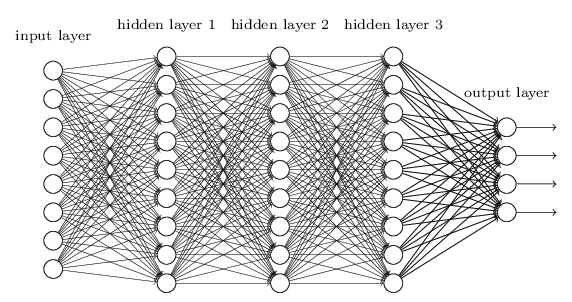
\includegraphics[width=1\linewidth]{../assets/decision-trees/diagrams/neural}
	
	\label{fig:neural}
\end{figure}
\end{frame}

\begin{frame}{Learnt Decision Tree}
\begin{tikzpicture}[
node/.style={%
	draw,
	rectangle,
},
]

\node [node] (A) {Outlook};
\path (A) ++(-150:\nodeDist) node [node] (B) {Humidity};
\path (A) ++(-90:\nodeDist/2) node [node, fill=green] (C) {Yes};
\path (A) ++(-30:\nodeDist) node [node] (D) {Wind};
\path (B) ++(-135:\nodeDist) node [node, fill=red] (E) {No};
\path (B) ++(-45:\nodeDist) node [node, fill=green] (F) {Yes};
\path (D) ++(-45:\nodeDist) node [node, fill=red] (G) {No};
\path (D) ++(-135:\nodeDist) node [node, fill=green] (H) {Yes};

\draw (A) -- (B) node [left,pos=0.25] {Sunny}(A);
\draw (A) -- (C) node [right,pos=0.8] {Overcast}(A);
\draw (A) -- (D) node [right,pos=0.5] {Rain}(A);
\draw (B) -- (E) node [left,pos=0.25] {High}(A);
\draw (B) -- (F) node [right,pos=0.25] {Normal}(C);
\draw (D) -- (G) node [right,pos=0.25] {Strong}(A);
\draw (D) -- (H) node [left,pos=0.25] {Weak}(A);
\end{tikzpicture}

\end{frame}

\begin{frame}{Medical Diagnosis using Decision Trees }
\begin{figure}
	\centering
	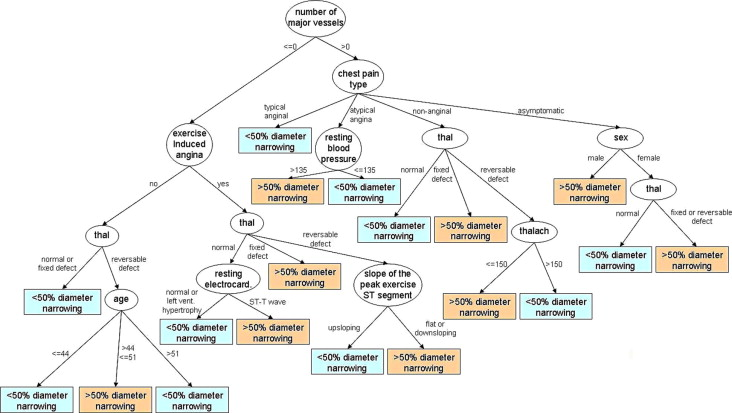
\includegraphics[width=1\linewidth]{../assets/decision-trees/diagrams/decision-medical}
	\caption{Source: Improving medical decision trees by combining relevant health-care criteria}
	\label{fig:decision-medical}
\end{figure}

\end{frame}


\begin{frame}{Leo Brieman}
\begin{figure}
	\centering
	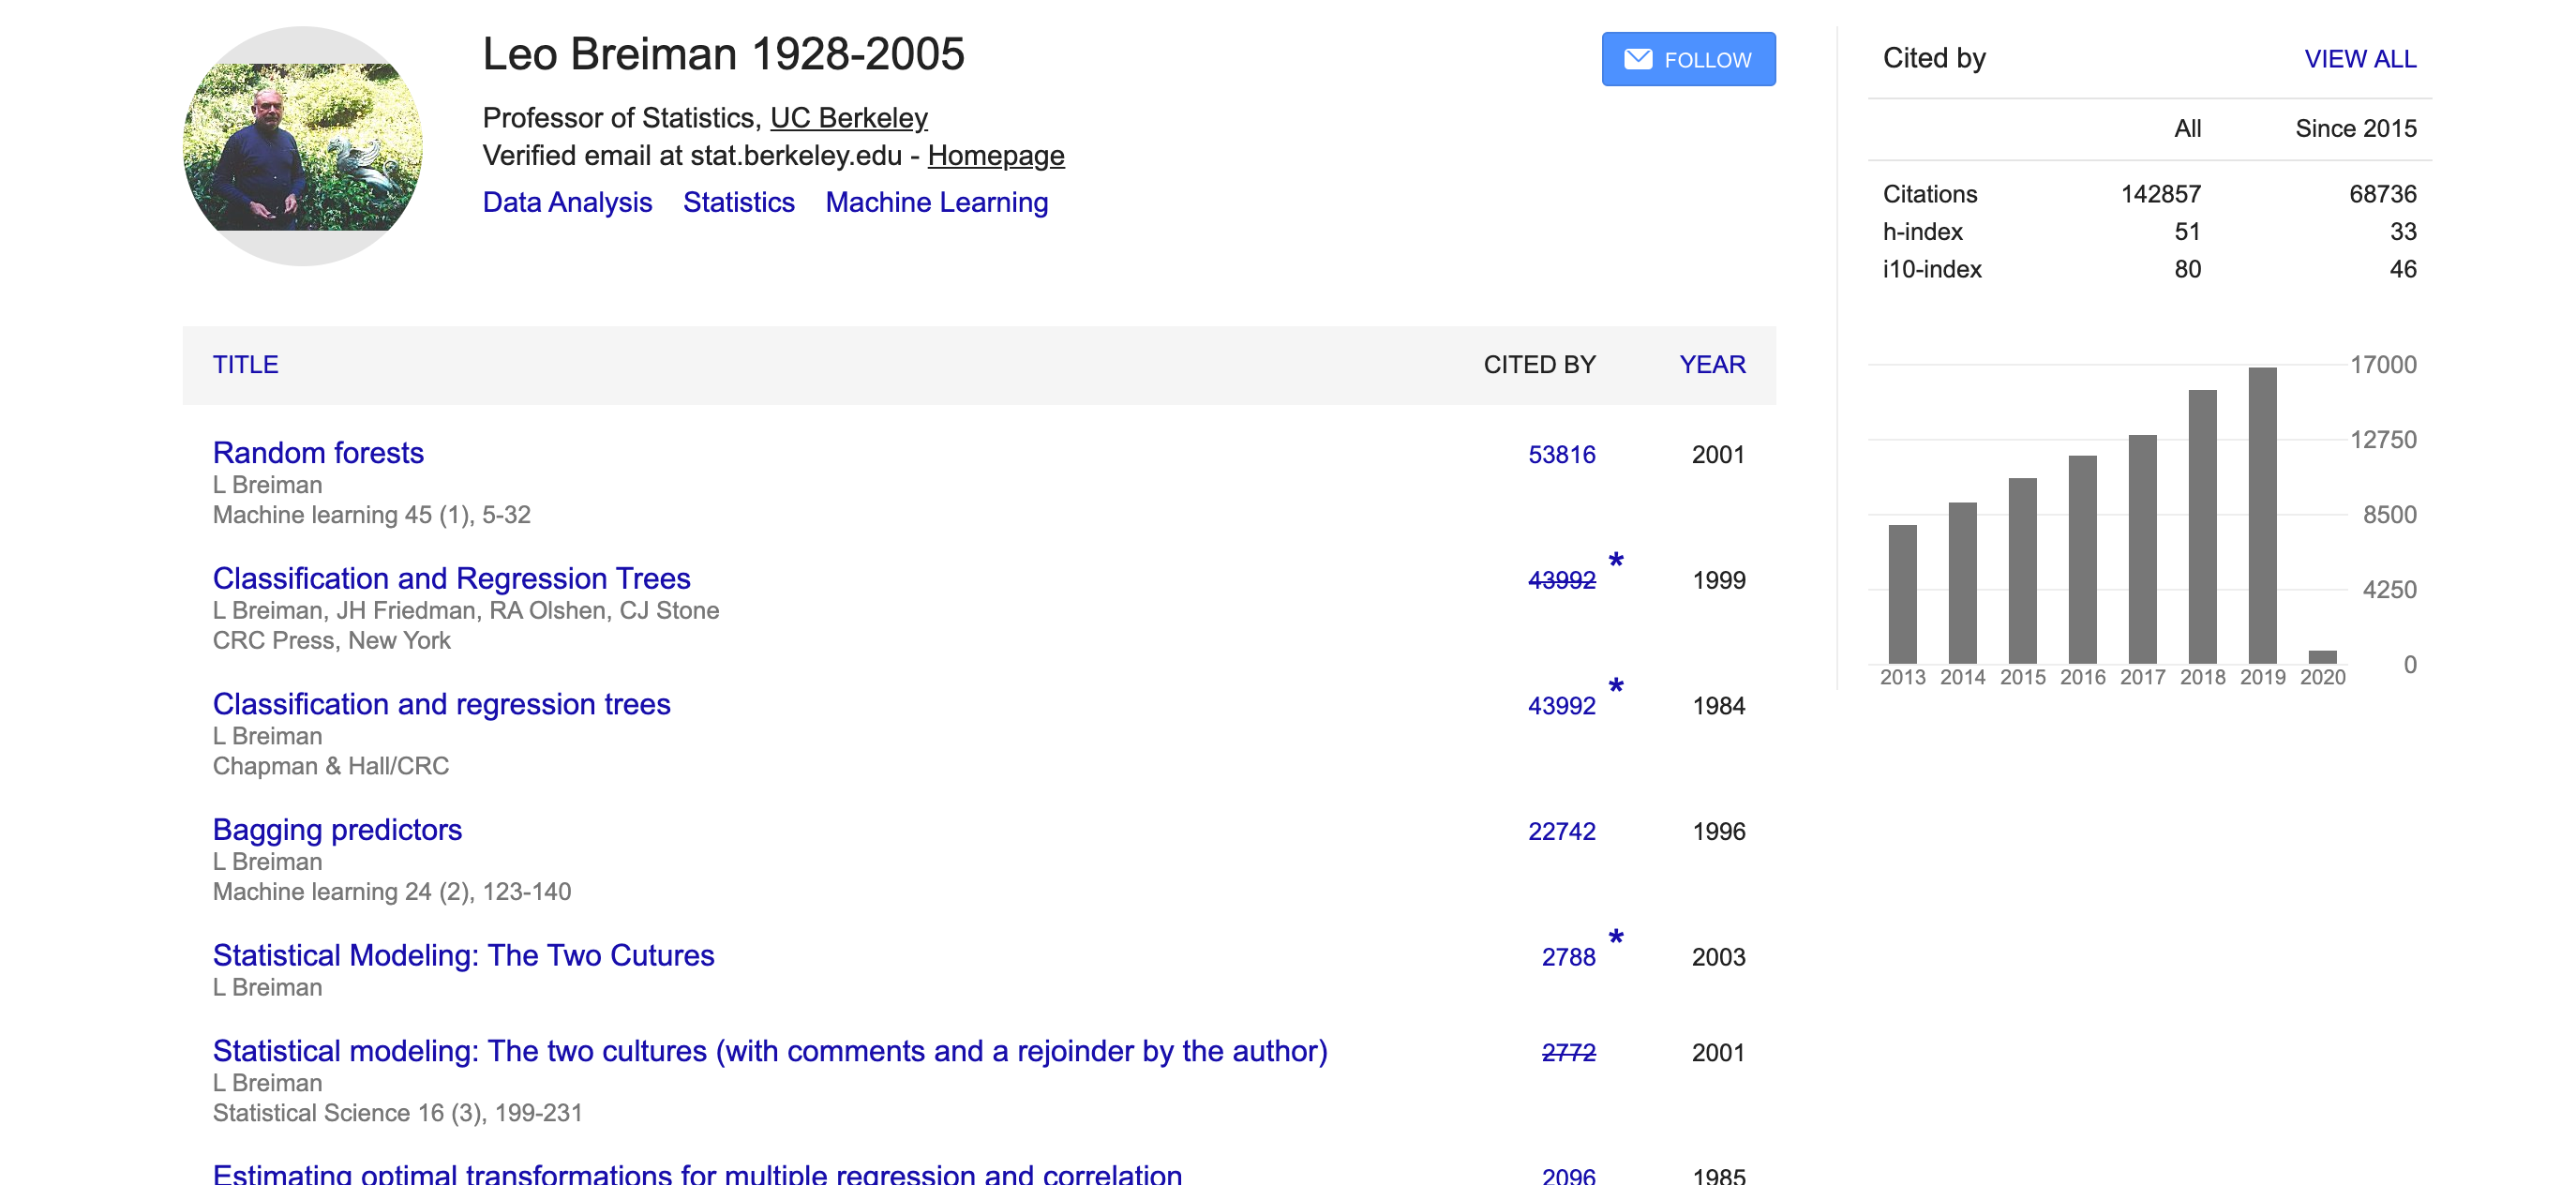
\includegraphics[width=1\linewidth]{../assets/decision-trees/diagrams/brieman}

	\label{fig:brieman}
\end{figure}

\end{frame}

\begin{frame}{Optimal Decision Tree}
\begin{figure}
	\centering
	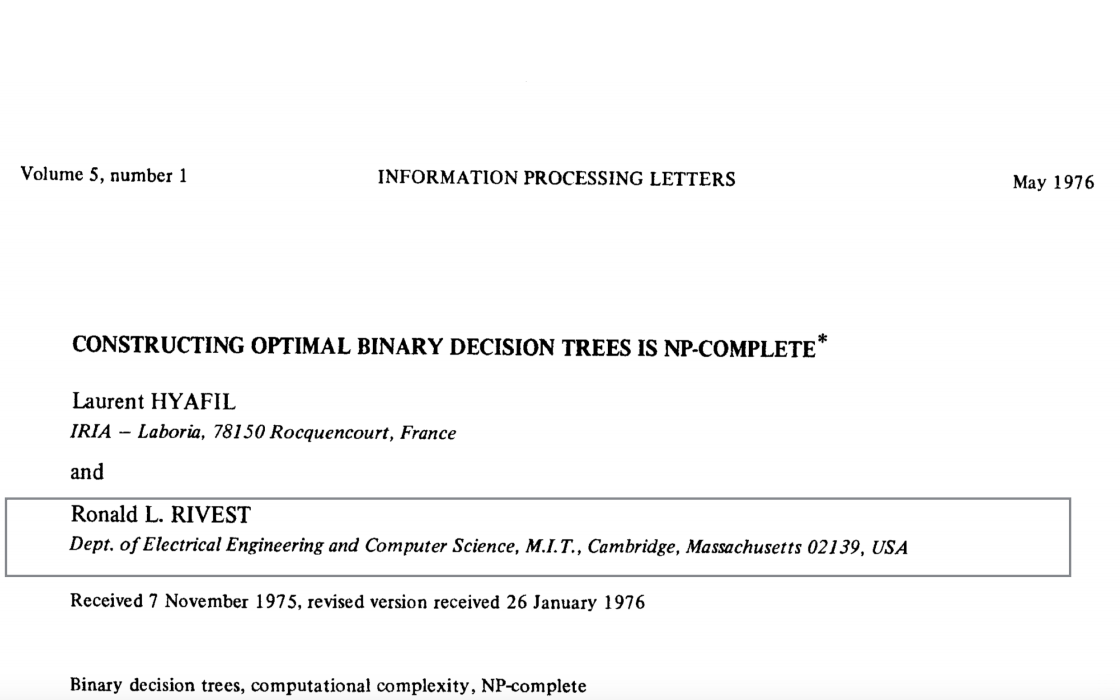
\includegraphics[width=1\linewidth]{../assets/decision-trees/diagrams/NP-hard}

	\label{fig:np-hard}
\end{figure}

\end{frame}

\begin{frame}{Greedy Algorithm}
Core idea: At each level, choose an attribute that gives
\textbf{biggest estimated} performance gain!

\begin{figure}
	\centering
	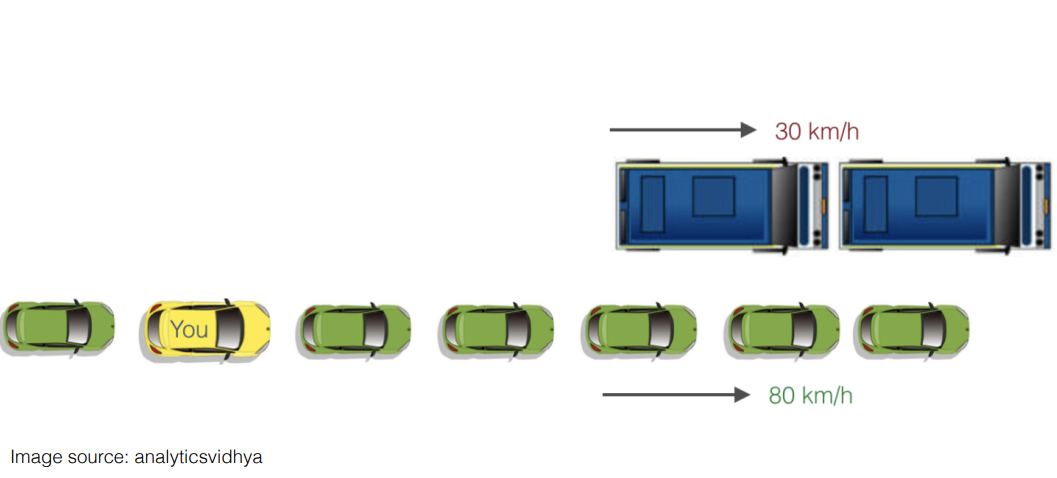
\includegraphics[width=0.8\linewidth]{../assets/decision-trees/diagrams/gredy}
	\caption{Greedy!=Optimal}
	\label{fig:gredy}
\end{figure}

\end{frame}

\begin{frame}{Towards biggest estimated performance gain}
\begin{columns}
\begin{column}{.7\textwidth}


\begin{scriptsize}


	\begin{tabular}{lllll||l} \toprule
	\textbf{Day} & \textbf{Outlook}  & \textbf{Temp} & \textbf{Humidity} & \textbf{Windy}  & \textbf{Play} \\ \midrule
	D1  & Sunny    & Hot  & High     & Weak   & No   \\
	D2  & Sunny    & Hot  & High     & Strong & No   \\
	D3  & Overcast & Hot  & High     & Weak   & Yes  \\
	D4  & Rain     & Mild & High     & Weak   & Yes  \\
	D5  & Rain     & Cool & Normal   & Weak   & Yes  \\
	D6  & Rain     & Cool & Normal   & Strong & No   \\
	D7  & Overcast & Cool & Normal   & Strong & Yes  \\
	D8  & Sunny    & Mild & High     & Weak   & No   \\
	D9  & Sunny    & Cool & Normal   & Weak   & Yes  \\
	D10 & Rain     & Mild & Normal   & Weak   & Yes  \\
	D11 & Sunny    & Mild & Normal   & Strong & Yes  \\
	D12 & Overcast & Mild & High     & Strong & Yes  \\
	D13 & Overcast & Hot  & Normal   & Weak   & Yes  \\
	D14 & Rain     & Mild & High     & Strong & No  \\ \bottomrule
\end{tabular}
\end{scriptsize}
\end{column}
\begin{column}{0.4\textwidth}
	\begin{scriptsize}
\begin{itemize}
	\pause \item For examples, we have 9 Yes, 5 No
	\pause \item Would it be trivial if we had 14 Yes or 14 No?
	\pause \item Yes!
	\pause \item Key insight: Problem is ``easier'' when there is less disagreement
	\pause 	\item Need some statistical measure of ``disagreement'' 
	\end{itemize}

\end{scriptsize}
\end{column}

\end{columns}

\end{frame}




%\begin{frame}
%\begin{forest}
%	for tree={grow'=south}
%	[Outlook
%	[Humidity, edge label={node[midway,fill=gray,font=\scriptsize]{Sunny}} []]
%	[Wind, edge label={node[midway,fill=white,font=\scriptsize]{Rain}} [] [] []]
%	[Yes, edge label={node[midway,fill=white,font=\scriptsize]{Overcast}}]
%	]
%\end{forest}
%\end{frame}

\begin{frame}{Entropy}
 Statistical measure to characterize the
(im)purity of examples

\pause $H(X) = -\sum_{i=1}^k p(x_i) \log_2 p(x_i)$

\begin{figure}[htp]
    \centering
    \begin{notebookbox}{https://nipunbatra.github.io/ml-teaching/notebooks/entropy.html}
      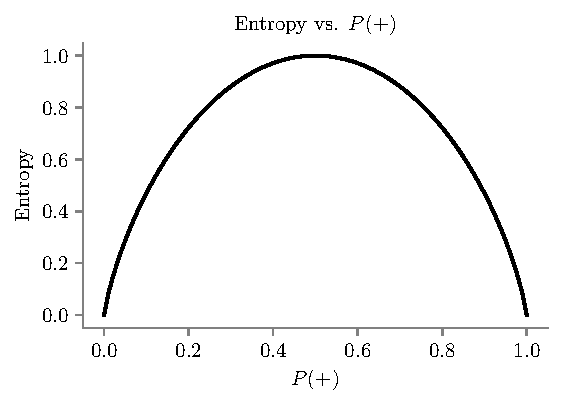
\includegraphics[scale=0.6]{../assets/decision-trees/figures/entropy.pdf}
    \end{notebookbox}
  \end{figure}

\end{frame}
	
\begin{frame}{Towards biggest estimated performance gain}
\begin{columns}
	\begin{column}{.7\textwidth}
		
		
		\begin{scriptsize}
			

			\begin{tabular}{lllll||l} \toprule
				\textbf{Day} & \textbf{Outlook}  & \textbf{Temp} & \textbf{Humidity} & \textbf{Windy}  & \textbf{Play} \\ \midrule
				D1  & Sunny    & Hot  & High     & Weak   & No   \\
				D2  & Sunny    & Hot  & High     & Strong & No   \\
				D3  & Overcast & Hot  & High     & Weak   & Yes  \\
				D4  & Rain     & Mild & High     & Weak   & Yes  \\
				D5  & Rain     & Cool & Normal   & Weak   & Yes  \\
				D6  & Rain     & Cool & Normal   & Strong & No   \\
				D7  & Overcast & Cool & Normal   & Strong & Yes  \\
				D8  & Sunny    & Mild & High     & Weak   & No   \\
				D9  & Sunny    & Cool & Normal   & Weak   & Yes  \\
				D10 & Rain     & Mild & Normal   & Weak   & Yes  \\
				D11 & Sunny    & Mild & Normal   & Strong & Yes  \\
				D12 & Overcast & Mild & High     & Strong & Yes  \\
				D13 & Overcast & Hot  & Normal   & Weak   & Yes  \\
				D14 & Rain     & Mild & High     & Strong & No  \\ \bottomrule
			\end{tabular}
		\end{scriptsize}
	\end{column}
	\begin{column}{0.4\textwidth}
		\begin{scriptsize}
			\begin{itemize}
				\pause \item Can we use Outlook as the root node?
				\pause 	\item When Outlook is overcast, we always Play and thus no ``disagreement'' 
			\end{itemize}
			
		\end{scriptsize}
	\end{column}
	
\end{columns}

\end{frame}
	
\begin{frame}{Information Gain}
 Reduction in entropy
by partitioning examples (S) on attribute A
$$
\operatorname{Gain}(S, A) \equiv \text{Entropy}(S)-\sum_{v \in \text{Values}(A)} \frac{|S_{v}|}{|S|} \text{Entropy}(S_{v})
$$
\end{frame}


\begin{frame}{ID3 (Examples, Target Attribute, Attributes)}
\begin{itemize}[<+->]
	\item Create a root node for tree
	\item If all examples are +/-, return root with label = +/-
	\item  If attributes = empty, return root with most common value of
	Target Attribute in Examples
	\item Begin
	\begin{itemize}[<+->]
		\item A $\leftarrow$ attribute from Attributes which best classifies
		Examples
		\item 	Root $\leftarrow$ A
		\item  For each value (v) of A
		\begin{itemize}[<+->]
			\item Add new tree branch : A = v
			\item  Examples\textsubscript{v}: subset of examples that A = v
			\item If Examples\textsubscript{v}is empty: add leaf with label = most
			common value of Target Attribute
			\item Else: ID3 (Examples\textsubscript{v}, Target attribute, Attributes - {A})
		\end{itemize}
	\end{itemize}


\end{itemize}
\end{frame}

\begin{frame}{Learnt Decision Tree}
\begin{tikzpicture}[
node/.style={%
	draw,
	rectangle,
},
]

\node [node] (A) {Root Node (empty)};

\end{tikzpicture}

\end{frame}

	\begin{frame}{Training Data}
\begin{tabular}{lllll||l} \toprule
	\textbf{Day} & \textbf{Outlook}  & \textbf{Temp} & \textbf{Humidity} & \textbf{Windy}  & \textbf{Play} \\ \midrule
	D1  & Sunny    & Hot  & High     & Weak   & No   \\
	D2  & Sunny    & Hot  & High     & Strong & No   \\
	D3  & Overcast & Hot  & High     & Weak   & Yes  \\
	D4  & Rain     & Mild & High     & Weak   & Yes  \\
	D5  & Rain     & Cool & Normal   & Weak   & Yes  \\
	D6  & Rain     & Cool & Normal   & Strong & No   \\
	D7  & Overcast & Cool & Normal   & Strong & Yes  \\
	D8  & Sunny    & Mild & High     & Weak   & No   \\
	D9  & Sunny    & Cool & Normal   & Weak   & Yes  \\
	D10 & Rain     & Mild & Normal   & Weak   & Yes  \\
	D11 & Sunny    & Mild & Normal   & Strong & Yes  \\
	D12 & Overcast & Mild & High     & Strong & Yes  \\
	D13 & Overcast & Hot  & Normal   & Weak   & Yes  \\
	D14 & Rain     & Mild & High     & Strong & No  \\ \bottomrule
\end{tabular}
\end{frame}


\begin{frame}{Entropy calculated}
We have 14 examples in $S$: 5 No, 9 Yes

$$\Entropy(S) = -p_{\text{No}} \log_2 p_{\text{No}} - p_{\text{Yes}} \log_2 p_{\text{Yes}}$$
$$
= -\frac{5}{14} \log_2\left(\frac{5}{14}\right) - \frac{9}{14} \log_2\left(\frac{9}{14}\right) = 0.940
$$
\end{frame}

\begin{frame}{Information Gain for Outlook}
\begin{tabular}{l|l} \toprule
\textbf{Outlook} & \textbf{Play} \\ \midrule
Sunny    & No   \\
Sunny    & No   \\
Overcast & Yes  \\
Rain     & Yes  \\
Rain     & Yes  \\
Rain     & No   \\
Overcast & Yes  \\
Sunny    & No   \\
Sunny    & Yes  \\
Rain     & Yes  \\
Sunny    & Yes  \\
Overcast & Yes  \\
Overcast & Yes  \\
Rain     & No  \\ \bottomrule
\end{tabular}
\end{frame}

\begin{frame}{Information Gain for Outlook}
\begin{columns}


\begin{column}{.32\textwidth}
	\begin{table}
\begin{tabular}{l|l} \toprule
	\textbf{Outlook} & \textbf{Play} \\ \midrule
	Sunny    & No   \\
	Sunny    & No   \\
	Sunny    & No   \\
	Sunny    & Yes  \\
	Sunny    & Yes  \\

\bottomrule
\end{tabular}
We have 2 Yes, 3 No
$\Entropy = -\frac{3}{5} \log_2\left(\frac{3}{5}\right) - \frac{2}{5} \log_2\left(\frac{2}{5}\right) = 0.971$
\end{table}
\end{column}

\pause \begin{column}{.32\textwidth}
	\begin{table}


\begin{tabular}{l|l} \toprule
	\textbf{Outlook} & \textbf{Play} \\ \midrule

	Overcast & Yes  \\
	Overcast & Yes  \\
	Overcast & Yes  \\
	Overcast & Yes  \\ \bottomrule

\end{tabular}
We have 4 Yes, 0 No
$\Entropy = 0$ (pure subset)


	\end{table}


\end{column}


\pause \begin{column}{.32\textwidth}
	\begin{table}
\begin{tabular}{l|l} \toprule
	\textbf{Outlook} & \textbf{Play} \\ \midrule
	Rain     & Yes  \\
	Rain     & Yes  \\
	Rain     & No   \\
	Rain     & Yes  \\
	Rain     & No  \\ \bottomrule
\end{tabular}
We have 3 Yes, 2 No
$\Entropy = -\frac{3}{5} \log_2\left(\frac{3}{5}\right) - \frac{2}{5} \log_2\left(\frac{2}{5}\right) = 0.971$
\end{table}
\end{column}
\end{columns}
\end{frame}

\begin{frame}{Information Gain}
$$
\operatorname{Gain}(S, \text{Outlook}) = \text{Entropy}(S)-\sum_{v \in \{\text{Rain, Sunny, Overcast}\}} \frac{|S_{v}|}{|S|} \text{Entropy}(S_{v}) 
$$

\begin{align}
\Gain(S, \text{Outlook}) &= \Entropy(S) - \frac{5}{14} \Entropy(S_{\text{Sunny}}) \\
&\quad - \frac{4}{14} \Entropy(S_{\text{Overcast}}) - \frac{5}{14} \Entropy(S_{\text{Rain}}) \\
&= 0.940 - \frac{5}{14} \times 0.971 - \frac{4}{14} \times 0 - \frac{5}{14} \times 0.971 \\
&= 0.940 - 0.347 - 0 - 0.347 = 0.246
\end{align}

\end{frame}

\begin{frame}{Information Gain}


\begin{tikzpicture}
\begin{axis}[
symbolic x coords={Outlook,Humidity,Wind,Temperature},
xtick=data,xtick pos=left, width=8cm,
ytick pos=left,axis x line*=bottom,nodes near coords,hide y axis,title=Information Gain, ymin=0.0]
\addplot[ybar,fill=black] coordinates {
	(Outlook,0.246)
	(Humidity,0.151)
	(Wind,0.048)
	(Temperature,0.029)
};
\end{axis}
\end{tikzpicture}


\end{frame}

\begin{frame}{Learnt Decision Tree}
\begin{tikzpicture}[
node/.style={%
	draw,
	rectangle,
},
]

\node [node] (A) {Outlook};
\path (A) ++(-150:\nodeDist) node [node] (B) {?};
\path (A) ++(-90:\nodeDist/2) node [node, fill=green] (C) {Yes};
\path (A) ++(-30:\nodeDist) node [node] (D) {?};


\draw (A) -- (B) node [left,pos=0.25] {Sunny}(A);
\draw (A) -- (C) node [right,pos=0.8] {Overcast}(A);
\draw (A) -- (D) node [right,pos=0.5] {Rain}(A);

\end{tikzpicture}

\end{frame}

	\begin{frame}{Calling ID3 on Outlook=Sunny}
\begin{tabular}{llll||l} \toprule
	\textbf{Day} & \textbf{Temp} & \textbf{Humidity} & \textbf{Windy}  & \textbf{Play} \\ \midrule
	D1    & Hot  & High     & Weak   & No   \\
	D2     & Hot  & High     & Strong & No   \\
	D8     & Mild & High     & Weak   & No   \\
	D9    & Cool & Normal   & Weak   & Yes  \\
	D11    & Mild & Normal   & Strong & Yes  \\ \bottomrule
\end{tabular}

\begin{itemize}
	\pause \item Gain($S_{\text{Outlook=Sunny}}$, Temp) = Entropy(2 Yes, 3 No) - (2/5)*Entropy(0 Yes, 2 No) -(2/5)*Entropy(1 Yes, 1 No) - (1/5)*Entropy(1 Yes, 0 No) 
	\pause \item Gain($S_{\text{Outlook=Sunny}}$, Humidity) = Entropy(2 Yes, 3 No) - (2/5)*Entropy(2 Yes, 0 No) -(3/5)*Entropy(0 Yes, 3 No) $\implies$ \textbf{maximum possible for the set}
	\pause \item Gain($S_{\text{Outlook=Sunny}}$, Windy) = Entropy(2 Yes, 3 No) - (3/5)*Entropy(1 Yes, 2 No) -(2/5)*Entropy(1 Yes, 1 No) 
\end{itemize}
\end{frame}

\begin{frame}{Learnt Decision Tree}
\begin{tikzpicture}[
node/.style={%
	draw,
	rectangle,
},
]

\node [node] (A) {Outlook};
\path (A) ++(-150:\nodeDist) node [node] (B) {Humidity};
\path (A) ++(-90:\nodeDist/2) node [node, fill=green] (C) {Yes};
\path (A) ++(-30:\nodeDist) node [node] (D) {?};
\path (B) ++(-135:\nodeDist) node [node, fill=red] (E) {No};
\path (B) ++(-45:\nodeDist) node [node, fill=green] (F) {Yes};
;

\draw (A) -- (B) node [left,pos=0.25] {Sunny}(A);
\draw (A) -- (C) node [right,pos=0.8] {Overcast}(A);
\draw (A) -- (D) node [right,pos=0.5] {Rain}(A);
\draw (B) -- (E) node [left,pos=0.25] {High}(A);
\draw (B) -- (F) node [right,pos=0.25] {Normal}(C);

\end{tikzpicture}

\end{frame}


	\begin{frame}{Calling ID3 on (Outlook=Rain)}
\begin{tabular}{llll||l} \toprule
	\textbf{Day}  & \textbf{Temp} & \textbf{Humidity} & \textbf{Windy}  & \textbf{Play} \\ \midrule
	D4    & Mild & High     & Weak   & Yes  \\
	D5     & Cool & Normal   & Weak   & Yes  \\
	D6      & Cool & Normal   & Strong & No   \\
	D10     & Mild & Normal   & Weak   & Yes  \\
	D14      & Mild & High     & Strong & No  \\ \bottomrule
\end{tabular}
\begin{itemize}
	\item The attribute Windy gives the highest information gain
\end{itemize}
\end{frame}

\begin{frame}{Learnt Decision Tree}
\begin{tikzpicture}[
node/.style={%
	draw,
	rectangle,
},
]

\node [node] (A) {Outlook};
\path (A) ++(-150:\nodeDist) node [node] (B) {Humidity};
\path (A) ++(-90:\nodeDist/2) node [node, fill=green] (C) {Yes};
\path (A) ++(-30:\nodeDist) node [node] (D) {Wind};
\path (B) ++(-135:\nodeDist) node [node, fill=red] (E) {No};
\path (B) ++(-45:\nodeDist) node [node, fill=green] (F) {Yes};
\path (D) ++(-45:\nodeDist) node [node, fill=red] (G) {No};
\path (D) ++(-135:\nodeDist) node [node, fill=green] (H) {Yes};

\draw (A) -- (B) node [left,pos=0.25] {Sunny}(A);
\draw (A) -- (C) node [right,pos=0.8] {Overcast}(A);
\draw (A) -- (D) node [right,pos=0.5] {Rain}(A);
\draw (B) -- (E) node [left,pos=0.25] {High}(A);
\draw (B) -- (F) node [right,pos=0.25] {Normal}(C);
\draw (D) -- (G) node [right,pos=0.25] {Strong}(A);
\draw (D) -- (H) node [left,pos=0.25] {Weak}(A);
\end{tikzpicture}

\end{frame}

\begin{frame}{Prediction for Decision Tree}
Just walk down the tree!

\begin{tikzpicture}[
node/.style={%
	draw,
	rectangle,
},
]

\node [node] (A) {Outlook};
\path (A) ++(-150:\nodeDist) node [node] (B) {Humidity};
\path (A) ++(-90:\nodeDist/2) node [node, fill=green] (C) {Yes};
\path (A) ++(-30:\nodeDist) node [node] (D) {Wind};
\path (B) ++(-135:\nodeDist) node [node, fill=red] (E) {No};
\path (B) ++(-45:\nodeDist) node [node, fill=green] (F) {Yes};
\path (D) ++(-45:\nodeDist) node [node, fill=red] (G) {No};
\path (D) ++(-135:\nodeDist) node [node, fill=green] (H) {Yes};

\draw (A) -- (B) node [left,pos=0.25] {Sunny}(A);
\draw (A) -- (C) node [right,pos=0.8] {Overcast}(A);
\draw (A) -- (D) node [right,pos=0.5] {Rain}(A);
\draw (B) -- (E) node [left,pos=0.25] {High}(A);
\draw (B) -- (F) node [right,pos=0.25] {Normal}(C);
\draw (D) -- (G) node [right,pos=0.25] {Strong}(A);
\draw (D) -- (H) node [left,pos=0.25] {Weak}(A);
\end{tikzpicture}

\pause Prediction for $<$High Humidity, Strong Wind, Sunny Outlook, Hot Temp$>$ is ? \\
\pause  No
\end{frame}

\begin{frame}{Limiting Depth of Tree}
Assuming if you were only allowed depth-$1$ trees, how would it look for the current dataset? \\

\pause Apply the same rules, except when depth limit is reached, the leaf node is assigned the most common occurring value in that path.

\pause What is depth-$0$ tree (no decision) for the examples? \\
\pause Always predicting Yes

\pause What is depth-$1$ tree (no decision) for the examples? \\
\pause \begin{tikzpicture}[
node/.style={%
	draw,
	rectangle,
},
]

\node [node] (A) {Outlook};
\path (A) ++(-150:\nodeDist) node [node, fill=red] (B) {No};
\path (A) ++(-90:\nodeDist/2) node [node, fill=green] (C) {Yes};
\path (A) ++(-30:\nodeDist) node [node, fill=green] (D) {Yes};


\draw (A) -- (B) node [left,pos=0.25] {Sunny}(A);
\draw (A) -- (C) node [right,pos=0.8] {Overcast}(A);
\draw (A) -- (D) node [right,pos=0.5] {Rain}(A);

\end{tikzpicture}

\end{frame}

\section{Discrete Input, Real Output}

\begin{frame}{Modified Dataset}
\begin{table}[]
	\begin{tabular}{@{}llllll@{}}
		\toprule
		\textbf{Day} & \textbf{Outlook} & \textbf{Temp} & \textbf{Humidity} & \textbf{Wind} & \textbf{Minutes Played} \\ \midrule
		D1           & Sunny            & Hot           & High              & Weak          & 20                      \\
		D2           & Sunny            & Hot           & High              & Strong        & 24                      \\
		D3           & Overcast         & Hot           & High              & Weak          & 40                      \\
		D4           & Rain             & Mild          & High              & Weak          & 50                      \\
		D5           & Rain             & Cool          & Normal            & Weak          & 60                      \\
		D6           & Rain             & Cool          & Normal            & Strong        & 10                      \\
		D7           & Overcast         & Cool          & Normal            & Strong        & 4                       \\
		D8           & Sunny            & Mild          & High              & Weak          & 10                      \\
		D9           & Sunny            & Cool          & Normal            & Weak          & 60                      \\
		D10          & Rain             & Mild          & Normal            & Weak          & 40                      \\
		D11          & Sunny            & Mild          & High              & Strong        & 45                      \\
		D12          & Overcast         & Mild          & High              & Strong        & 40                      \\
		D13          & Overcast         & Hot           & Normal            & Weak          & 35                      \\
		D14          & Rain             & Mild          & High              & Strong        & 20                      \\ \bottomrule
	\end{tabular}
\end{table}
\end{frame}

\begin{frame}{Measure of Impurity for Regression?}
\begin{itemize}
	\item \pause Any guesses?
	\item \pause Mean Squared Error
	\item \pause $\MSE(S) = 311.34$
	\item \pause What about splitting criterion for regression?
	\item \pause \textbf{MSE Reduction} (not Information Gain!)
	\item \pause MSE Reduction = $\MSE(S) - \sum_{v} \frac{|S_v|}{|S|} \MSE(S_v)$
\end{itemize}

\end{frame}

\begin{frame}{Gain by splitting on Wind}
\begin{columns}

\begin{column}{.5\textwidth}
	\begin{scriptsize}

\begin{table}[]
	\begin{tabular}{@{}ll@{}}
		\toprule
		\textbf{Wind} & \textbf{Minutes Played} \\ \midrule
		Weak          & 20                      \\
		Strong        & 24                      \\
		Weak          & 40                      \\
		Weak          & 50                      \\
		Weak          & 60                      \\
		Strong        & 10                      \\
		Strong        & 4                       \\
		Weak          & 10                      \\
		Weak          & 60                      \\
		Weak          & 40                      \\
		Strong        & 45                      \\
		Strong        & 40                      \\
		Weak          & 35                      \\
		Strong        & 20                      \\ \bottomrule
	\end{tabular}
\caption{MSE(S)=311.34}
\end{table}
	\end{scriptsize}
\end{column}
\begin{column}{.5\textwidth}
	\begin{tiny}
\vspace{-5pt}		
\begin{table}[]
	\begin{tabular}{@{}ll@{}}
		\toprule
		\textbf{Wind} & \textbf{Minutes Played} \\ \midrule
		Weak          & 20                      \\
		Weak          & 40                      \\
		Weak          & 50                      \\
		Weak          & 60                      \\
		Weak          & 10                      \\
		Weak          & 60                      \\
		Weak          & 40                      \\
		Weak          & 35                      \\ \bottomrule
	\end{tabular}
\caption{$\MSE(S_{\text{Wind=Weak}}) = 277$, Weight = $\frac{8}{14}$}
\end{table}
\vspace{-25pt}
	\end{tiny}

	\begin{tiny}
	
	\begin{table}[]
		\begin{tabular}{@{}ll@{}}
			\toprule
			\textbf{Wind} & \textbf{Minutes Played} \\ \midrule

			Strong        & 24                      \\
			Strong        & 10                      \\
			Strong        & 4                       \\
			Strong        & 45                      \\
			Strong        & 40                      \\
			Strong        & 20                      \\ \bottomrule
		\end{tabular}
\caption{$\MSE(S_{\text{Wind=Strong}}) = 218$, Weight = $\frac{6}{14}$}
	\end{table}
\end{tiny}

\end{column}
\end{columns}
\end{frame}

\begin{frame}{MSE Reduction Calculation}
\textbf{Correct calculation for Wind split:}
\begin{align}
\text{MSE Reduction} &= \MSE(S) - \text{Weighted Average MSE} \\
&= 311.34 - \left[\frac{8}{14} \times 277 + \frac{6}{14} \times 218\right] \\
&= 311.34 - [158.857 + 93.429] \\
&= 311.34 - 252.286 = \mathbf{59.05}
\end{align}

\textbf{Key insight:} MSE Reduction $> 0$ means the split improves our model!

\textbf{For regression:} Use MSE Reduction, NOT Information Gain!
\end{frame}

\begin{frame}{MSE Reduction for Regression Trees}

	\begin{figure}[htp]
		\centering
		\begin{notebookbox}{https://nipunbatra.github.io/ml-teaching/notebooks/decision-tree-real-output.html}
		  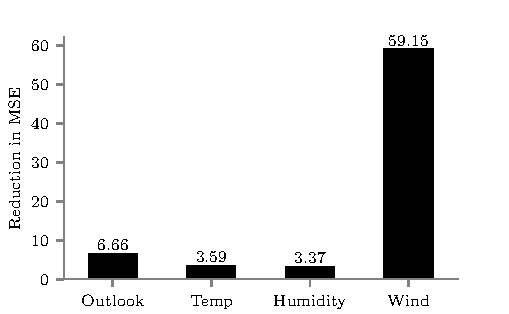
\includegraphics[width=\linewidth]{../assets/decision-trees/figures/discrete-input-real-output-level-1.pdf}
		\end{notebookbox}
	  \end{figure}

\end{frame}

\begin{frame}{Learnt Tree}
\begin{figure}
	\centering
	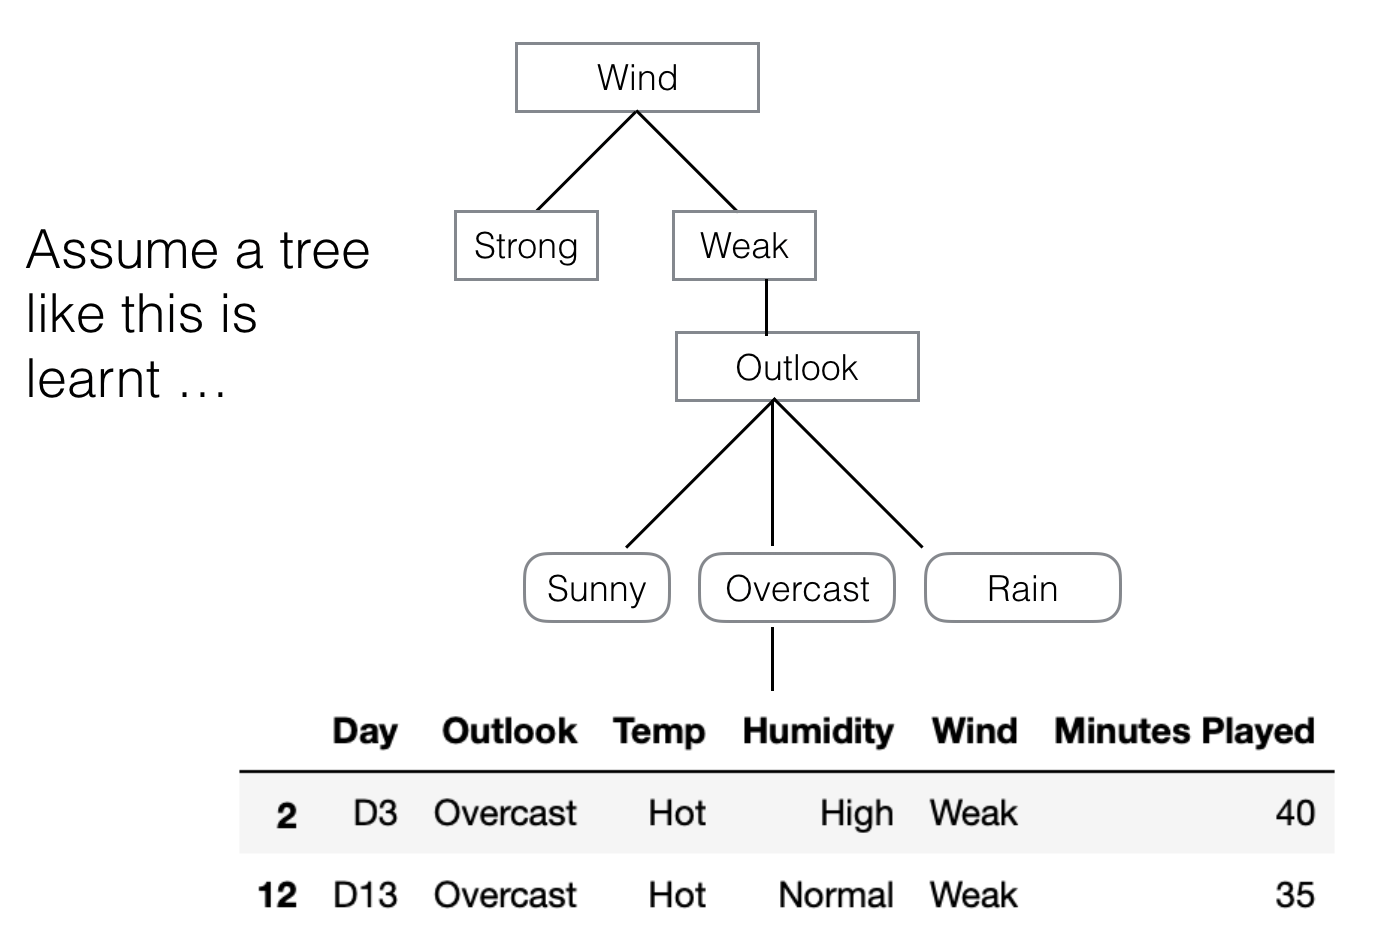
\includegraphics[width=1\linewidth]{../assets/decision-trees/diagrams/tree}

	\label{fig:tree}
\end{figure}

\end{frame}

\begin{frame}{Learnt Tree}
\begin{figure}
	\centering
	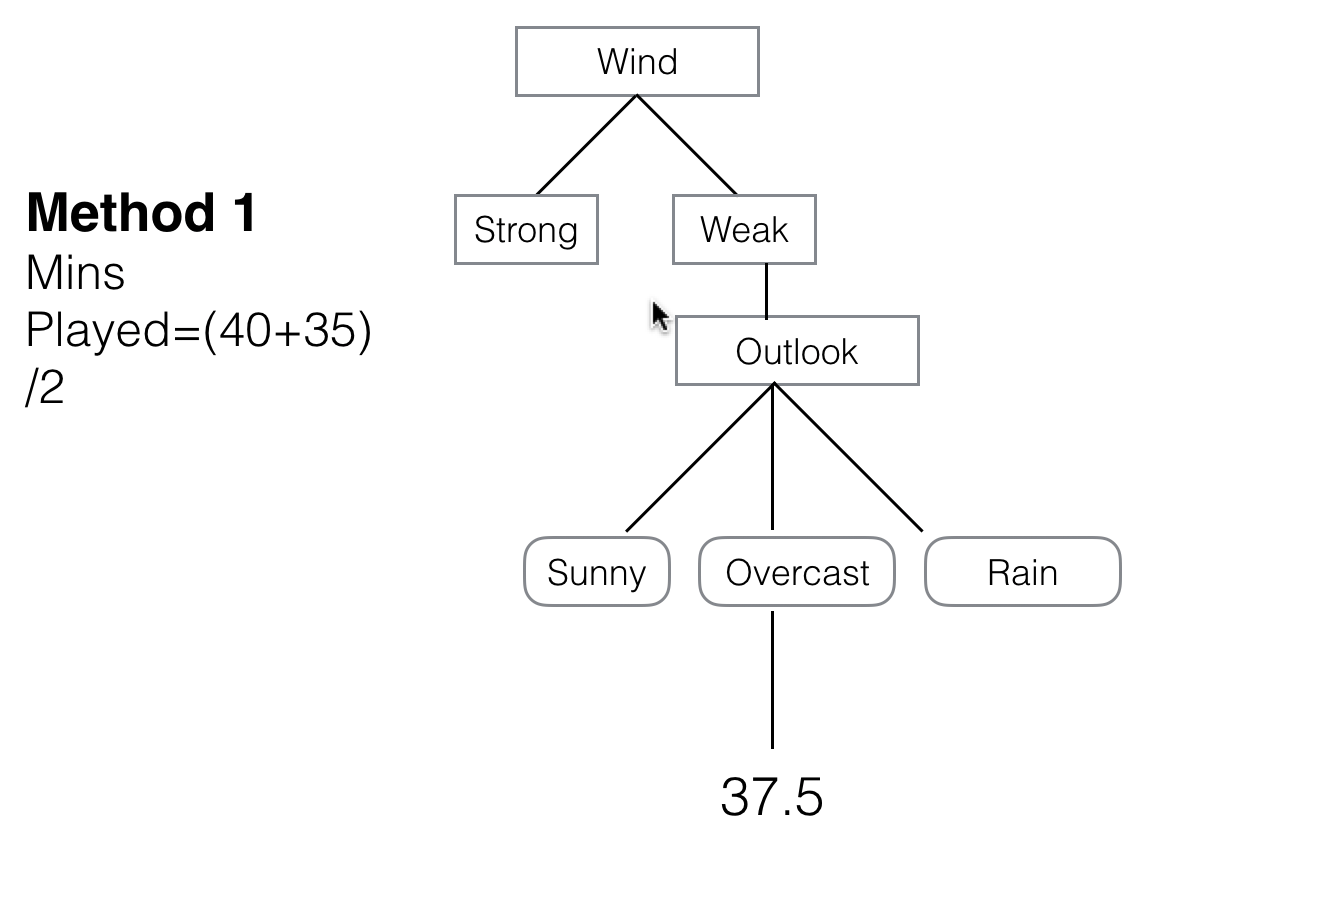
\includegraphics[width=1\linewidth]{../assets/decision-trees/diagrams/tree2}

	\label{fig:tree}
\end{figure}

\end{frame}

\section{Real Input Discrete Output}


\begin{frame}{Finding splits}
\begin{table}[]
	\begin{tabular}{@{}lrr@{}}
		\toprule
		\textbf{Day} & \textbf{Temperature} & \textbf{PlayTennis} \\ \midrule
		D1           & 40                   & No                  \\
		D2           & 48                   & No                  \\
		D3           & 60                   & Yes                 \\
		D4           & 72                   & Yes                 \\
		D5           & 80                   & Yes                 \\
		D6           & 90                   & No                  \\ \bottomrule
	\end{tabular}
\end{table}
\begin{itemize}[<+->]
	\item How do you find splits?
	\item Sort by attribute
	\item Find potential split points (midpoints). 
	\item For the above example, we have 5 potential splits: 44, 54, 66, 76, 85
	\item Calculate the weighted impurity for each split
	\item Choose the split with the lowest impurity
\end{itemize}
\end{frame}

\begin{frame}{Finding splits}
	\begin{table}[]
		\begin{tabular}{@{}lrr@{}}
			\toprule
			\textbf{Day} & \textbf{Temperature} & \textbf{PlayTennis} \\ \midrule
			D1           & 40                   & No                  \\
			D2           & 48                   & No                  \\
			D3           & 60                   & Yes                 \\
			D4           & 72                   & Yes                 \\
			D5           & 80                   & Yes                 \\
			D6           & 90                   & No                  \\ \bottomrule
		\end{tabular}
	\end{table}
	\begin{itemize}
		\item Consider split at 44
		\item LHS has 1 No and 0 Yes; RHS has 3 Yes and 2 No
		\item Entropy for LHS = 0, Entropy for RHS = 0.971
		\item Weighted Entropy = 0.971*5/6 = 0.808
	\end{itemize}
	\end{frame}

	\begin{frame}{Finding splits}
		\begin{table}[]
			\begin{tabular}{@{}lrr@{}}
				\toprule
				\textbf{Day} & \textbf{Temperature} & \textbf{PlayTennis} \\ \midrule
				D1           & 40                   & No                  \\
				D2           & 48                   & No                  \\
				D3           & 60                   & Yes                 \\
				D4           & 72                   & Yes                 \\
				D5           & 80                   & Yes                 \\
				D6           & 90                   & No                  \\ \bottomrule
			\end{tabular}
		\end{table}
		\begin{itemize}
			\item Consider split at 54
			\item LHS has 2 No and 0 Yes; RHS has 3 Yes and 1 No
			\item Entropy for LHS = 0, Entropy for RHS = 0.811
			\item Weighted Entropy = 0.811*4/6 = 0.541
		\end{itemize}
		\end{frame}

		\begin{frame}{Finding splits}
			\begin{table}[]
				\begin{tabular}{@{}lrr@{}}
					\toprule
					\textbf{Day} & \textbf{Temperature} & \textbf{PlayTennis} \\ \midrule
					D1           & 40                   & No                  \\
					D2           & 48                   & No                  \\
					D3           & 60                   & Yes                 \\
					D4           & 72                   & Yes                 \\
					D5           & 80                   & Yes                 \\
					D6           & 90                   & No                  \\ \bottomrule
				\end{tabular}
			\end{table}
			\begin{itemize}
				\item Consider split at 66
				\item LHS has 2 No and 1 Yes; RHS has 2 Yes and 1 No
				\item Entropy for LHS = 0.918, Entropy for RHS = 0.918
				\item Weighted Entropy = 0.918*3/6 + 0.918*3/6 = 0.918
			\end{itemize}
			\end{frame}


		\begin{frame}{Finding splits}
			\begin{table}[]
				\begin{tabular}{@{}lrr@{}}
					\toprule
					\textbf{Day} & \textbf{Temperature} & \textbf{PlayTennis} \\ \midrule
					D1           & 40                   & No                  \\
					D2           & 48                   & No                  \\
					D3           & 60                   & Yes                 \\
					D4           & 72                   & Yes                 \\
					D5           & 80                   & Yes                 \\
					D6           & 90                   & No                  \\ \bottomrule
				\end{tabular}
			\end{table}
			\begin{itemize}
				\item Consider split at 76
				\item LHS has 2 No and 2 Yes; RHS has 1 Yes and 1 No
				\item Entropy for LHS = 1, Entropy for RHS = 1
				\item Weighted Entropy = 1*4/6 + 1*2/6 = 1
			\end{itemize}
			\end{frame}

			\begin{frame}{Finding splits}
				\begin{table}[]
					\begin{tabular}{@{}lrr@{}}
						\toprule
						\textbf{Day} & \textbf{Temperature} & \textbf{PlayTennis} \\ \midrule
						D1           & 40                   & No                  \\
						D2           & 48                   & No                  \\
						D3           & 60                   & Yes                 \\
						D4           & 72                   & Yes                 \\
						D5           & 80                   & Yes                 \\
						D6           & 90                   & No                  \\ \bottomrule
					\end{tabular}
				\end{table}
				\begin{notebookbox}{https://nipunbatra.github.io/ml-teaching/notebooks/decision-tree-real-input-discrete-output.html}
					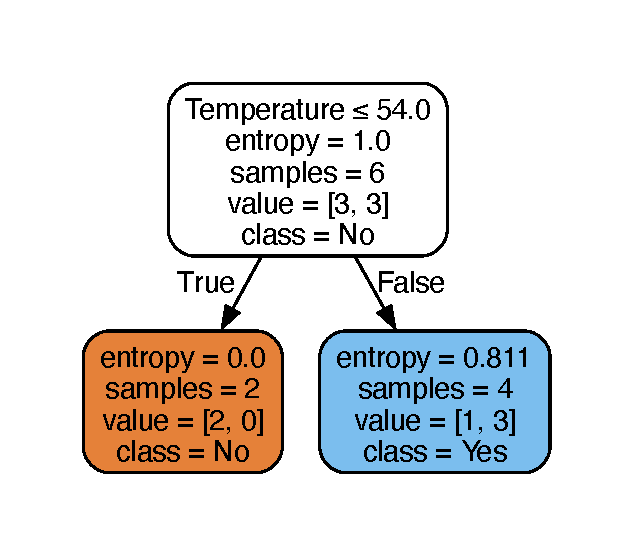
\includegraphics[scale=0.3]{../assets/decision-trees/figures/real-ip-1.pdf}
				\end{notebookbox}
				\end{frame}

				\begin{frame}{Finding splits}
					\begin{table}[]
						\begin{tabular}{@{}lrr@{}}
							\toprule
							\textbf{Day} & \textbf{Temperature} & \textbf{PlayTennis} \\ \midrule
							D1           & 40                   & No                  \\
							D2           & 48                   & No                  \\
							D3           & 60                   & Yes                 \\
							D4           & 72                   & Yes                 \\
							D5           & 80                   & Yes                 \\
							D6           & 90                   & No                  \\ \bottomrule
						\end{tabular}
					\end{table}
					\begin{notebookbox}{https://nipunbatra.github.io/ml-teaching/notebooks/decision-tree-real-input-discrete-output.html}
						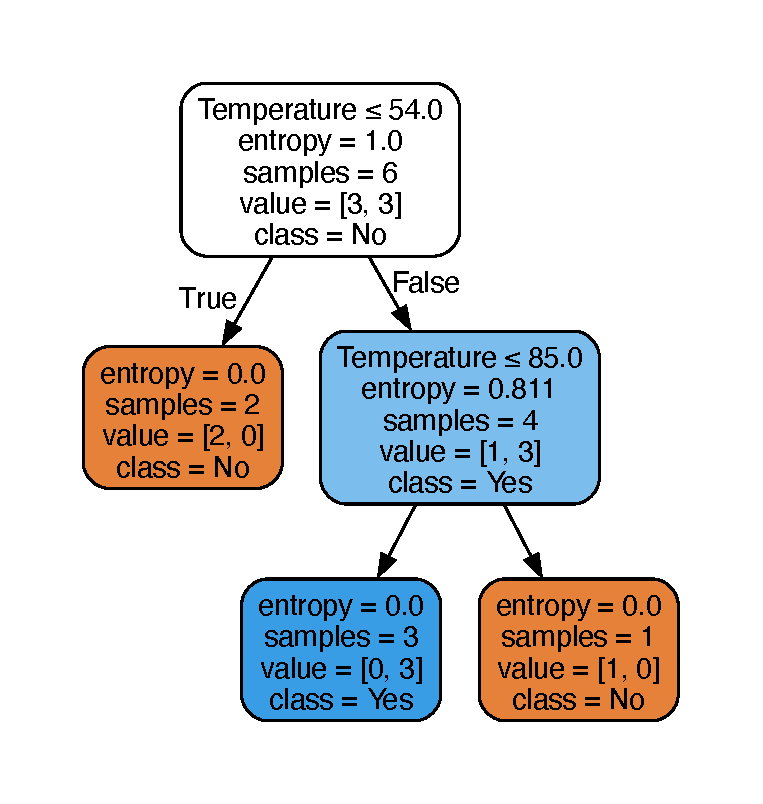
\includegraphics[scale=0.25]{../assets/decision-trees/figures/real-ip-2.pdf}
					\end{notebookbox}
					\end{frame}

\foreach \i in {1,...,9} {
\begin{frame}{Example (DT of depth \i)}
    \begin{figure}
		\centering
		\begin{notebookbox}{https://nipunbatra.github.io/ml-teaching/notebooks/decision-tree-real-input-discrete-output.html}
			\includegraphics{../assets/decision-trees/figures/dt-\i.pdf}
		  \end{notebookbox}
    
    \end{figure}
\end{frame}
}






\section{Real Input Real Output}

\begin{frame}{Example 1}
Let us consider the dataset given below
\begin{center}
	\begin{notebookbox}{https://nipunbatra.github.io/ml-teaching/notebooks/decision-tree-real-input-real-output.html}
		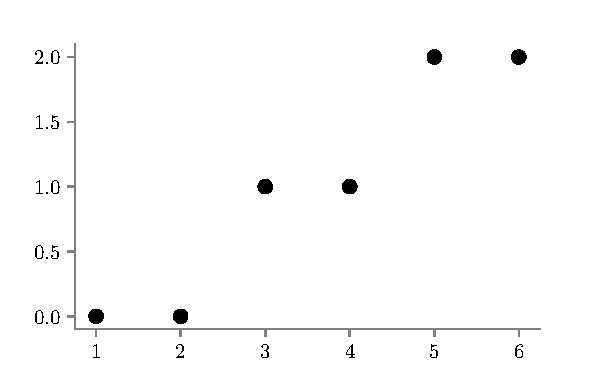
\includegraphics{../assets/decision-trees/figures/ri-ro-dataset.pdf}
	  \end{notebookbox}
\end{center}
\end{frame}

\begin{frame}{Example 1}
What would be the prediction for decision tree with depth 0?
\begin{center}
	\begin{notebookbox}{https://nipunbatra.github.io/ml-teaching/notebooks/decision-tree-real-input-real-output.html}
		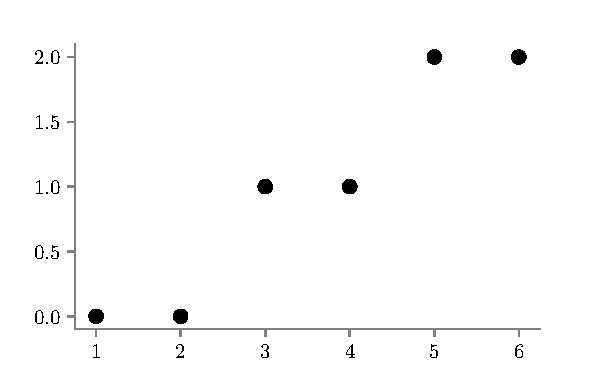
\includegraphics{../assets/decision-trees/figures/ri-ro-dataset.pdf}
	  \end{notebookbox}
\end{center}
\end{frame}

\begin{frame}{Example 1}
Prediction for decision tree with depth 0.\\
Horizontal dashed line shows the predicted $Y$ value. It is the average of $Y$ values of all datapoints.\\
\begin{center}
	\begin{notebookbox}{https://nipunbatra.github.io/ml-teaching/notebooks/decision-tree-real-input-real-output.html}
		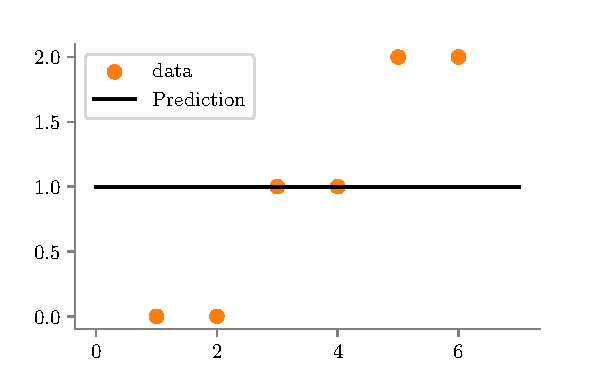
\includegraphics{../assets/decision-trees/figures/ri-ro-depth-0.pdf}	
	  \end{notebookbox}
\end{center}
\end{frame}


\begin{frame}{Example 1}
What would be the decision tree with depth 1?
\begin{center}
	\begin{notebookbox}{https://nipunbatra.github.io/ml-teaching/notebooks/decision-tree-real-input-real-output.html}
		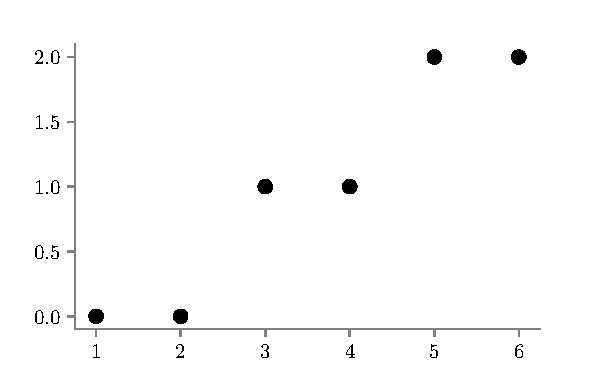
\includegraphics{../assets/decision-trees/figures/ri-ro-dataset.pdf}
	  \end{notebookbox}
\end{center}
\end{frame}

\begin{frame}{Example 1}
Decision tree with depth 1
\begin{center}
	\begin{notebookbox}{https://nipunbatra.github.io/ml-teaching/notebooks/decision-tree-real-input-real-output.html}
		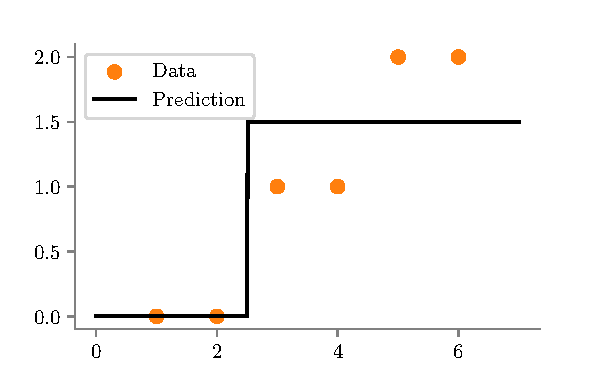
\includegraphics{../assets/decision-trees/figures/ri-ro-depth-1.pdf}
	\end{notebookbox}	
\end{center}
\end{frame}

\begin{frame}{Example 1}
The Decision Boundary
\begin{center}
	\begin{notebookbox}{https://nipunbatra.github.io/ml-teaching/notebooks/decision-tree-real-input-real-output.html}
		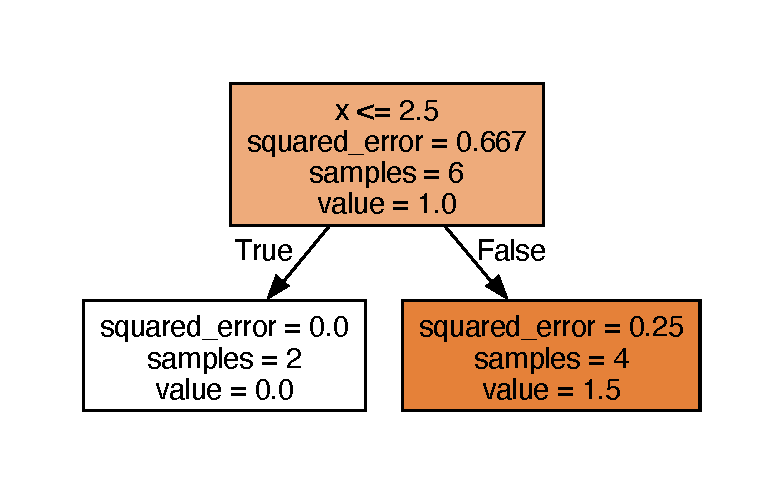
\includegraphics[scale=0.6]{../assets/decision-trees/figures/ri-ro-depth-1-sklearn.pdf}
	\end{notebookbox}
\end{center}
\end{frame}


\begin{frame}{Example 1}
What would be the decision tree with depth 2	?
\begin{center}
	\begin{notebookbox}{https://nipunbatra.github.io/ml-teaching/notebooks/decision-tree-real-input-real-output.html}
		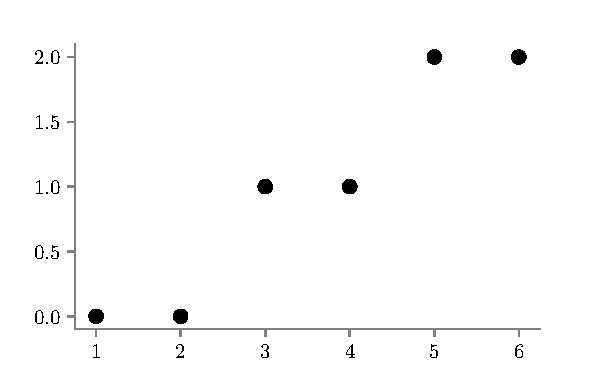
\includegraphics{../assets/decision-trees/figures/ri-ro-dataset.pdf}
	  \end{notebookbox}
\end{center}
\end{frame}

\begin{frame}{Example 1}
	Decision tree with depth 1
	\begin{center}
		\begin{notebookbox}{https://nipunbatra.github.io/ml-teaching/notebooks/decision-tree-real-input-real-output.html}
			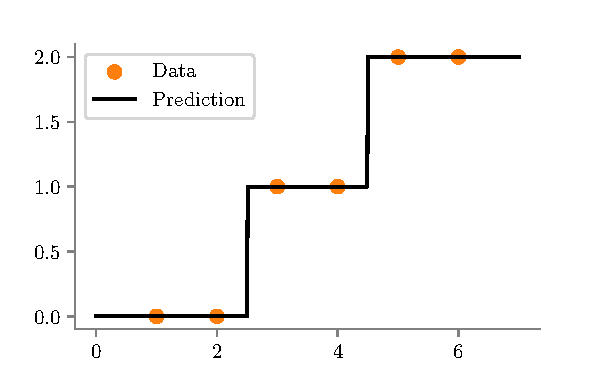
\includegraphics{../assets/decision-trees/figures/ri-ro-depth-2.pdf}
		\end{notebookbox}
	\end{center}
	\end{frame}
	
	\begin{frame}{Example 1}
	The Decision Boundary
	\begin{center}
		\begin{notebookbox}{https://nipunbatra.github.io/ml-teaching/notebooks/decision-tree-real-input-real-output.html}
			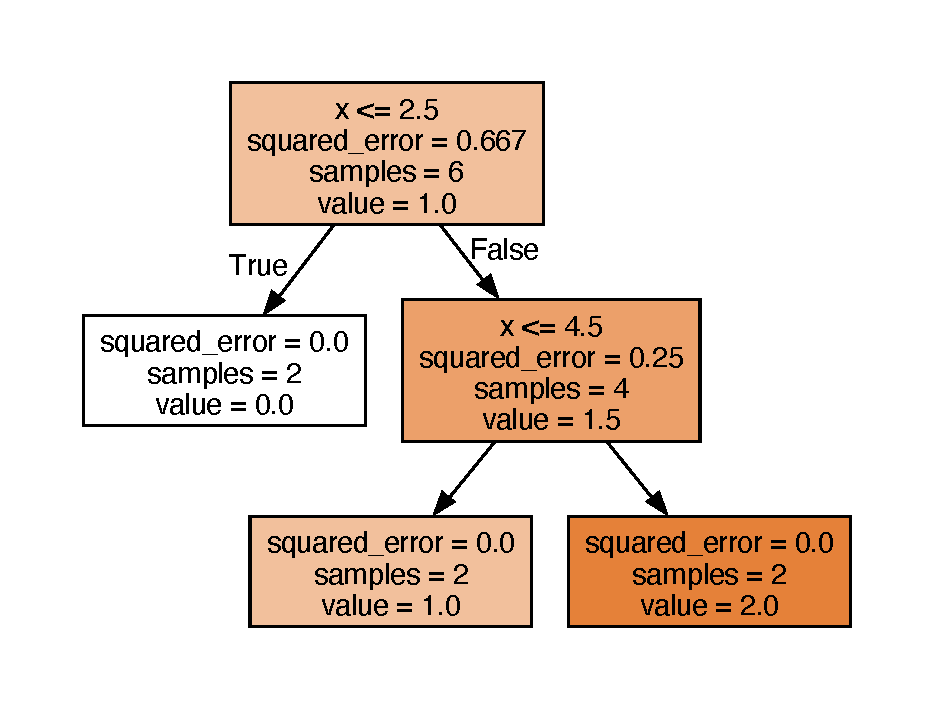
\includegraphics[scale=0.6]{../assets/decision-trees/figures/ri-ro-depth-2-sklearn.pdf}
		\end{notebookbox}
	\end{center}
	\end{frame}
	

\begin{frame}{Objective Function for Regression Trees}
\only<1-4>{
Feature is denoted by $X$ and target by $Y$.\\
Let the split be at $X = s$.\\
Define regions: $R_1 = \{x : x \leq s\}$ and $R_2 = \{x : x > s\}$.\\
\vspace{1cm}
}
\only<2-4>{
For each region, compute the mean prediction:\\
$c_1 = \frac{1}{|R_1|} \sum_{x_i \in R_1} y_i$ \\
$c_2 = \frac{1}{|R_2|} \sum_{x_i \in R_2} y_i$ \\
}
\only<3-4>{
The loss function is:\\
$$\text{Loss}(s) = \sum_{x_i \in R_1} (y_i - c_1)^2 + \sum_{x_i \in R_2} (y_i - c_2)^2$$
\vspace{1cm}
}
\only<4>{
Our objective is to find the optimal split:\\
$$s^* = \argmin_{s} \left[ \sum_{x_i \in R_1(s)} (y_i - c_1(s))^2 + \sum_{x_i \in R_2(s)} (y_i - c_2(s))^2 \right]$$
}
\end{frame}

\begin{frame}{Algorithm: Finding the Optimal Split}
\begin{enumerate}
\only<1-2>{
\item Sort all data points $(x_i, y_i)$ in increasing order of $x_i$.
\vspace{0.5cm}
}
\only<2>{
\item Evaluate the loss function for all candidate splits:
\vspace{0.25cm}
\begin{center}
$s = \frac{x_i + x_{i+1}}{2}$ for $i = 1, 2, \ldots, n-1$
\end{center}
\vspace{0.25cm}
\item Select the split $s^*$ that minimizes the loss function.
}
\end{enumerate} 
\end{frame}

\begin{frame}{A Question!}
Draw a regression tree for Y = sin(X), $0 \leq X \leq 2\pi$ 
\end{frame}

\begin{frame}{A Question!}
Dataset of Y = sin(X), $0 \leq X \leq 7$ with 10,000 points 
\begin{center}
	\begin{notebookbox}{https://nipunbatra.github.io/ml-teaching/notebooks/decision-tree-real-input-real-output.html}
		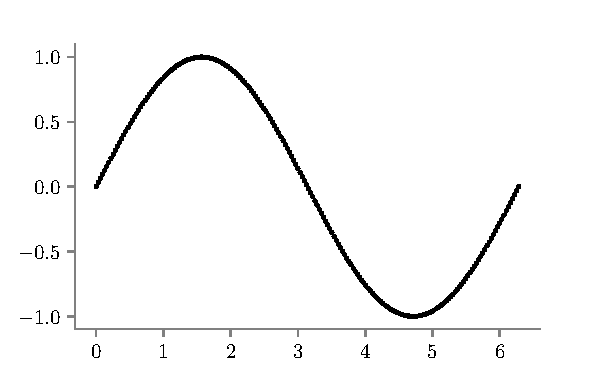
\includegraphics{../assets/decision-trees/figures/sine-dataset.pdf}
	  \end{notebookbox}
\end{center}
\end{frame}

\begin{frame}{A Question!}
Regression tree of depth 1
\begin{center}
	\begin{notebookbox}{https://nipunbatra.github.io/ml-teaching/notebooks/decision-tree-real-input-real-output.html}
		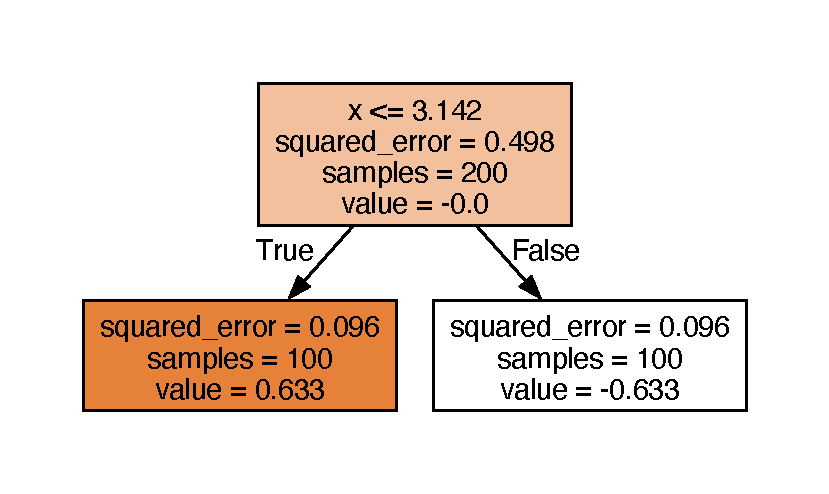
\includegraphics[scale=0.6]{../assets/decision-trees/figures/sine-depth-1-sklearn.pdf}
	  \end{notebookbox}
\end{center}
\end{frame}

\begin{frame}{A Question!}
Decision Boundary
\begin{center}
	\begin{notebookbox}{https://nipunbatra.github.io/ml-teaching/notebooks/decision-tree-real-input-real-output.html}
		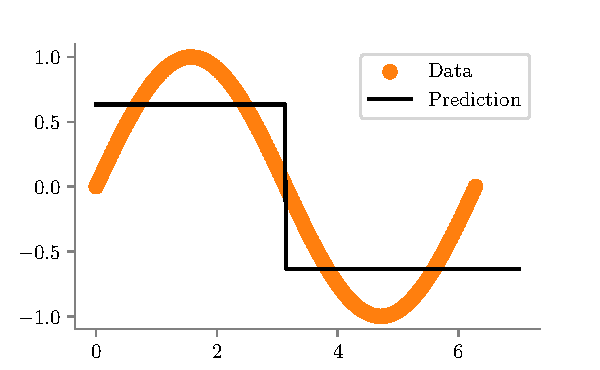
\includegraphics{../assets/decision-trees/figures/sine-depth-1.pdf}
	  \end{notebookbox}
\end{center}
\end{frame}

\begin{frame}{A Question!}
Regression tree with no depth limit is too big to fit in a slide. \\
It has of depth 4. The decision boundaries are in figure below.\\
\begin{center}
	\begin{notebookbox}{https://nipunbatra.github.io/ml-teaching/notebooks/decision-tree-real-input-real-output.html}
		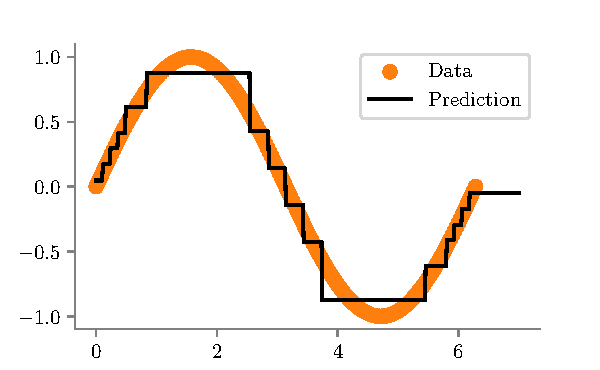
\includegraphics{../assets/decision-trees/figures/sine-depth-4.pdf}
	  \end{notebookbox}
\end{center}
\end{frame}

\begin{frame}{Summary}
\begin{itemize}
	\item Interpretability an important goal
\item Decision trees: well known interpretable models
\item  Learning optimal tree is hard
\item  Greedy approach:
\item  Recursively split to maximize “performance gain”
\item  Issues:
\begin{itemize}
	\item Can overfit easily!
	\item  Empirically not as powerful as other methods
\end{itemize}
\end{itemize}

\end{frame}


\begin{frame}

	\begin{figure}
		\centering
		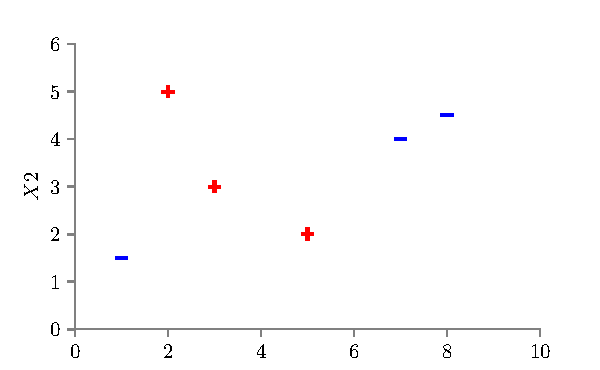
\includegraphics{../assets/decision-trees/figures/dt_weighted/fig1.pdf}
	\end{figure}
	
	
	\end{frame}
	
	
	\begin{frame}
	
	\begin{figure}
		\centering
		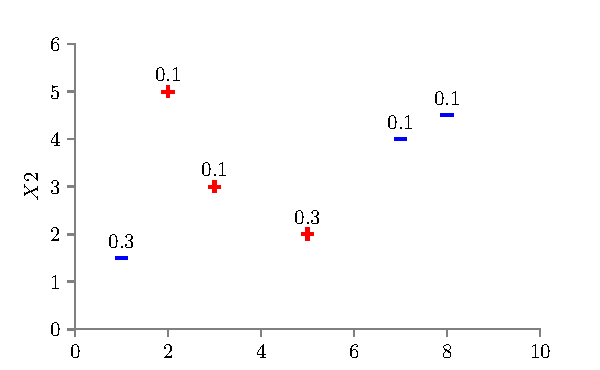
\includegraphics{../assets/decision-trees/figures/dt_weighted/fig2.pdf}
	\end{figure}
	
	
	\end{frame}
	
	
	\begin{frame}
	
	\begin{figure}
		\centering
		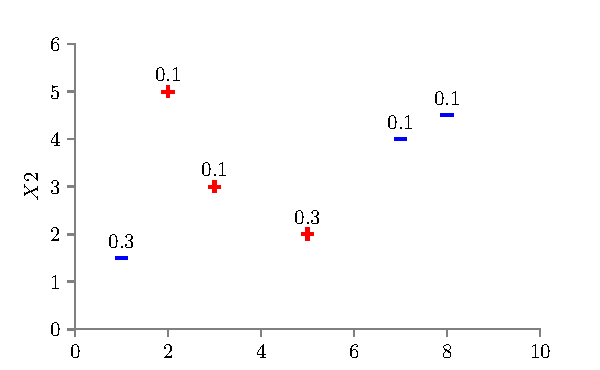
\includegraphics{../assets/decision-trees/figures/dt_weighted/fig2.pdf}
	\end{figure}
	
	$$\Entropy = -P(+) \log_2 P(+) - P(-) \log_2 P(-)$$
	
	$$P(+) = \frac{0.1 + 0.1 + 0.3}{1} = 0.5, \quad P(-) = \frac{0.3 + 0.1 + 0.1}{1} = 0.5$$
	
	$$\Entropy = E_s = -\frac{1}{2} \log_2 \frac{1}{2} - \frac{1}{2} \log_2 \frac{1}{2} = 1$$
	
	\end{frame}
	
	
	\begin{section}{Weighted Entropy}
	
	
	
	\begin{frame}
	
	\begin{figure}
		\centering
		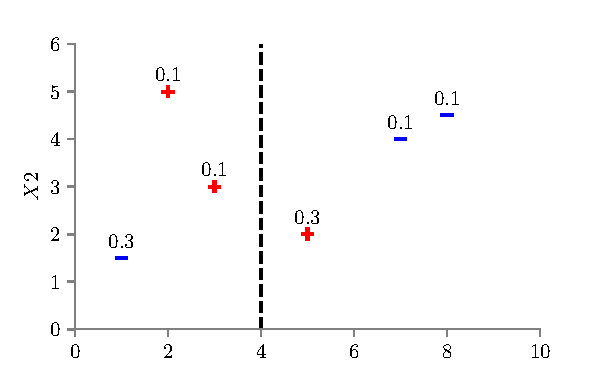
\includegraphics{../assets/decision-trees/figures/dt_weighted/fig3.pdf}
	\end{figure}
	
	
	Candidate Line: \(X1 = 4 (X1^*)\)
	
	
	\end{frame}
	
	
	\begin{frame}
	\begin{figure}
		\centering
		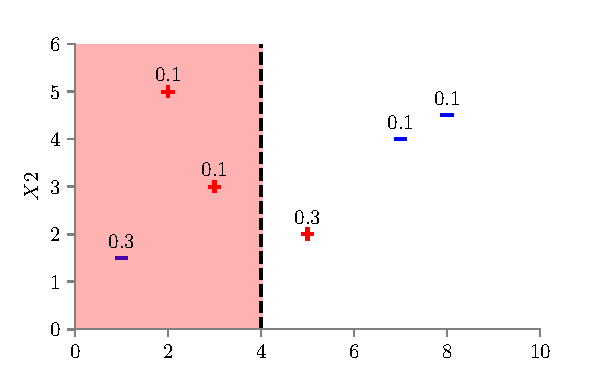
\includegraphics{../assets/decision-trees/figures/dt_weighted/fig4.pdf}
	\end{figure}
	
	Entropy of \(X1 \leq X1^*  = E_{S(X1 < X1^*)}\)
	
	$$P(+) = \frac{0.1 + 0.1}{0.1 + 0.1 + 0.3} = \frac{2}{5}$$
	
	$$P(-) = \frac{3}{5}$$
	
	
	\end{frame}
	
	
	\begin{frame}
	
	\begin{figure}
		\centering
		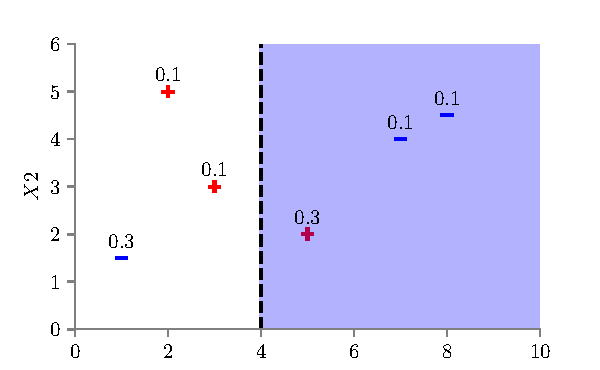
\includegraphics{../assets/decision-trees/figures/dt_weighted/fig5.pdf}
	\end{figure}
	Entropy of $X_1 > X_1^* = E_{S(X_1 > X_1^*)}$
	
	$$P(+) = \frac{3}{5}$$
	
	$$P(-) = \frac{2}{5}$$
	
	\end{frame}
	
	
	
	\begin{frame}
	
	\begin{figure}
		\centering
		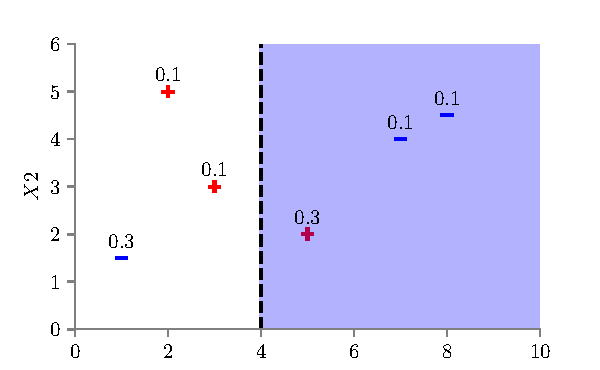
\includegraphics{../assets/decision-trees/figures/dt_weighted/fig5.pdf}
	\end{figure}
	
	$$\text{IG}(X_1 = X_1^*) = E_S - \frac{0.5}{1} \cdot E_{S(X_1 < X_1^*)} - \frac{0.5}{1} \cdot E_{S(X_1 > X_1^*)}$$
	
	\end{frame}

\end{section}
\end{document}
